\chapter{Verification of Message-Based Systems} \label{chap:design}
This chapter provides an in-depth discussion into the design decisions that were made during the development of Verlixir. The chapter will begin by providing a high-level overview of where the relevant components fit into the toolchain, as well as providing an architectural overview of the tool. Section \ref{sec:modelling_elixir_programs} will describe the main techniques Verlixir applies in the analysis and modelling of a specification and section \ref{sec:specification_language} will discuss the design of the LTLixir specifiation language. Finally, section \ref{sec:simulation_verification} will describe how the outputs generated by Verlixir are derived.  
\section{Verlixir Toolchain} \label{sec:toolchain}
We will first introduce where the new tools fit into the greater toolchain. Figure \ref{fig:high_level} shows a high-level overview of the toolchain. Given an LTLixir specification, either, the Elixir program can be compiled and run on the ERTS, or the program can be modelled by Verlixir and verified with Spin.
\begin{figure}[H]
    \centering
    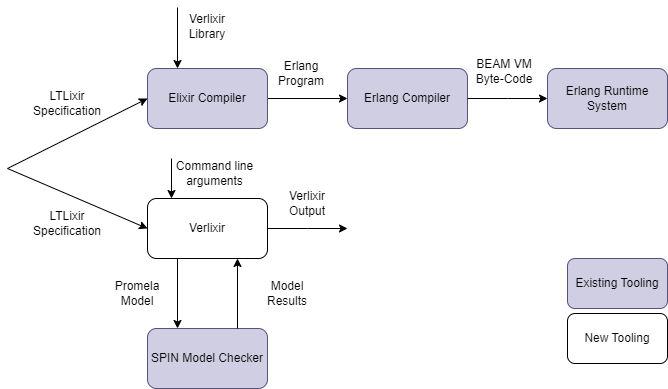
\includegraphics[width=0.9\textwidth]{images/high_level_system_v2.drawio.png}
    \caption{High-level overview of the verifiable Elixir toolchain.}
    \label{fig:high_level}
\end{figure}
Figure \ref{fig:low_level} provides an in-depth insight into the architecture underlying Verlixir.
\begin{figure}[H]
    \centering
    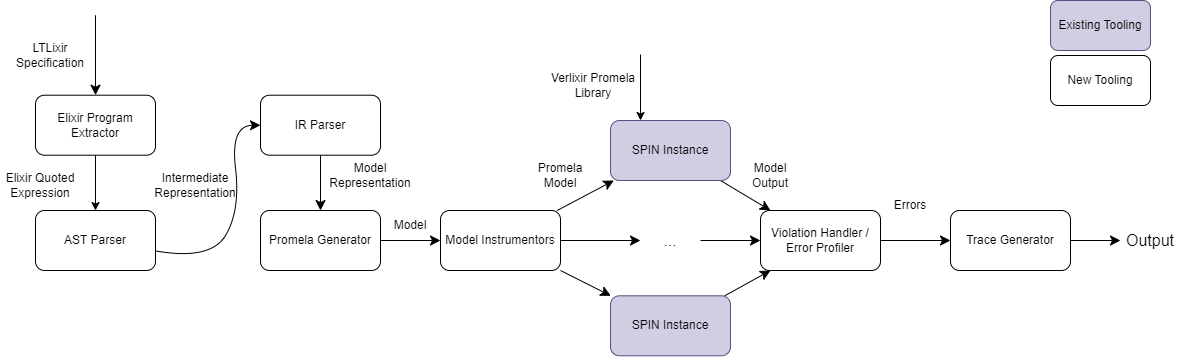
\includegraphics[width=1\textwidth]{images/detailed_diagram_v2.drawio.png}
    \caption{Verlixir design.}
    \label{fig:low_level}
\end{figure}
Before we discuss the design of Verlixir, we will summarise the components of the tool.
\begin{itemize}
    \item \textbf{LTLixir Specification}: Specification of an Elixir program to be parsed by Verlixir.
    \item \textbf{Elixir Extractor}: Converts the Elixir program into a quoted expression.
    \item \textbf{AST Parser}: Parses the quoted expression into an intermediate representation.
    \item \textbf{IR Parser}: Parses the intermediate representation, collecting relevant information for the model generator.
    \item \textbf{Promela Generator}: Writes a Promela model from the intermediate representation.
    \item \textbf{Model Instrumentors}: Instruments the model for appropriate verification (depending on system and user requirements).
    \item \textbf{Violation Handler}: Handles the output of the model checker by mapping violations back to the original Elixir program.
    \item \textbf{Trace Generator}: Generates an error trace from the mapped Elixir violations.
\end{itemize}
We briefly mention the technologies used in the design of the Verlixir artifact. Alongside the core Verlixir system, we introduce an Elixir library and a Promela library. 
\\ \\
The Elixir library is imported into programs that wish to access the LTLixir specification constructs we have introduced. In particular, contracts and predicates. The library is written in Elixir, using metaprogramming. With the library, comes the Elixir program extractor. The extractor, is an Elixir module, that converts Elixir syntax into a parsable quoted expression.
\\ \\
The Promela library is a hybrid between Promela and C. It is required to extend Promela beyond its basic capabilities; aligning it with the Elixir program semantics. The model generator uses the Promela library to model some Elixir constructs, for example, functions, data structures, message passing and more. Promela compiles models to C, so a C library incurs no overhead. However, C code can not be model-checked.
\\ \\
The core Verlixir offering (intermediate representation and Promela generator) is written in Rust. Rust is highly performant and provides software reliability guarantees that are relevant in asserting the correctness of the tool. Rust is highly optimised for parallelism, which we rely upon for optimising the model-checking process.
\section{Modelling Elixir Programs} \label{sec:modelling_elixir_programs}
The primary work done by Verlixir is determining how to internally represent an Elixir program. Given an Elixir program, with an inlined specification following the LTLixir semantics, Verlixir must both model the system and the properties of the specification. This section will outline the techniques used to achieve this.
\subsection{High-level Overview}
The internals of how the system is used to produce models of Elixir programs can be categorised into three umbrellas:
\begin{itemize}
    \item \textbf{Parsing}: takes an Elixir program and generates a quoted expression. Then, lexical analysis is performed on the quoted expression.
    \item \textbf{Intermediate Representation}: takes the parsed expression and generates an intermediate representation by extracting features relevant to model the program and specification.
    \item \textbf{Writing}: takes the intermediate representation and generates a model in a target language.
\end{itemize} 
The writer currently only supports the generation of Promela models, which can be verified using the model checker Spin, see section \ref{sec:simulation_verification}. Although this component of Verlixir can be split into these three stages, as they all work to achieve the same goal we will treat them as one and consider this component the \texttt{model generator}. 
\\ \\
To help understand the model generator, we begin by providing a high-level mapping of the supported set of Elixir constructs to Promela in table \ref{table:translation}.
\\ \\
\begin{longtable}{|>{\raggedright\arraybackslash}p{4cm}|>{\raggedright\arraybackslash}p{4cm}|>{\raggedright\arraybackslash}p{6cm}|}
    \hline
        \textbf{Elixir Expression} & \textbf{Promela Expression} & \textbf{Definition} \\
        \hline
        Functions & Processes & Every function call (recursive or else) spawns a new process. Function calls always block the parent process. If a function returns a value, the caller will await a rendezvous with the callee. \\
        \hline
        Process spawning & Processes & Process spawning translates naturally to Promela, using the $run$ keyword. \\
        \hline
        Boolean / arithmetic expressions & Expressions & The translation, for the supported set of operators, is direct to Promela for basic data types. Data structures, like lists, have custom inline code fragments for supported operators. \\
        \hline
        Matching (=) & Declaration, assignment & The first match in scope is translated as a declaration. Subsequent matches are re-assignments. In the case where the left-hand expression of a match is non-basic (i.e. tuple), a stack may be used to determine declaration ordering. \\
        \hline
        Types (integer, boolean, atom) & int, bool, mtype & Basic types include integers and booleans. Atoms are treated as message types (mtypes) and are globally unique. \\
        \hline
        Lists & Dynamically-sized arrays & Promela arrays have been extended to support dynamically sized lists. \\
        \hline
        For comprehensions & For loops &  A for comprehension over a range of values, translate to a Promela for loop. More complex comprehensions typically involve inlines. \\
        \hline
        If statements & If statements & If statements translate directly, with additional instrumentation as Promela blocks until a condition is matched. \\
        \hline
        Send & Channel append (!!) & A message will be packed into a new message structure, and then appended to the relevant mailbox channel. \\
        \hline
        Receive & Channel receive (??) & Receive involves matching the correct mailbox and message type. We can then remove the message from the channel and unpack the values. \\
        \hline
        LTL & LTL & Promela supports LTL. However, any variables or Elixir expressions present have to be specially translated before we translate the LTL formula. \\
        \hline
        Contracts & Assertions & Assertions are placed in process entry and exit points to ensure correctness. \\
        \hline
        Predicates & Global inlines & Predicates are recursively searched and moved to the global scope as inlines. \\
        \hline
    \caption{Overview of the translation of Elixir Expressions to Promela.}
    \label{table:translation}
\end{longtable}
The remainder of this section will discuss the techniques applied in the model generator, and specifically how the generator targets Promela as an output language.
\subsection{Sequential Execution} \label{sec:sequential_execution}
First, we explore how to model sequential execution. Elixir relies on a few parent identifiers that generally describe the structure of a program. We discuss a few flavours of these:
\begin{itemize}
    \item \textbf{Blocks}: blocks are a simple but core concept. An Elixir block contains multiple Elixir expressions separated by newlines or semi-colons.
    \item \textbf{Do}: Elixir control structures such as $if$ and $receive$ all use the $do$ keyword for a new expression. The child expression could be a single expression or a nested block.
    \item \textbf{Functions}: functions are essentially named or anonymous blocks, that can be spawned as processes.
    \item \textbf{Modules}: multiple functions can be grouped in a module. All Elixir code runs inside processes, so typically grouping functions in a module is a way to group functions that are related to the task a process performs.
\end{itemize}
These three constructs are examples of the primary building blocks of an Elixir program. With each, a new level of scope is introduced. Declared variables from parent scopes are accessible in child scopes, but any match to re-assign a variable from the parent scope will not persist. Instead, the structure of an Elixir program expects you to match the variable to the child scope, and return the intended assignment to the parent scope. Assuming there is no assignment to these constructs, then constructing a model is straightforward. We can derive the parent-child hierarchy directly. We hold multiple types of symbol tables, to represent the different constructs such as modules, functions and blocks. Within these symbol table types, we further can assign child symbol tables to account for the nesting of these scoped constructs.
\\ \\
\begin{figure}[h]
    \centering
    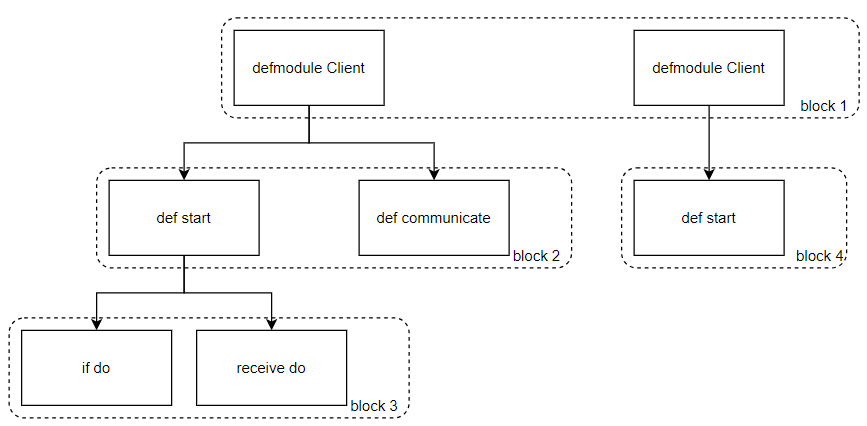
\includegraphics[width=0.8\textwidth]{images/sym_Table.png}
    \caption{An example symbol table scope hierarchy.}
    \label{fig:scope_hierarchy}
\end{figure}
\\ \\
\subsubsection{Traversal, Scoping and Variable Declarations}
So far, we assumed no expressions were matched to variables. To support assignment, we are required to track the execution of a scope in more detail. In the intermediate representation, a match is represented as either a \textbf{declaration} or an \textbf{assignment}. Given a declaration, we can infer the variable type and assign this in the symbol table. Now the variable is declared, any subsequent match in the same scope level is considered an assignment.
\\ \\
If we now match an expression that introduces a new child scope (such as a receive or if), we must explore every possible branch, determine the \textbf{returning expression} of the branch and use the relevant identifiers to assign the return value to the parent scope. To achieve this, the expression is traversed using a depth-first search with a stack of lists. The stack manages the scope nesting and the lists manage the variable identifiers. Let's explore an example.
\begin{lstlisting}[language=Elixir, xleftmargin=.1\linewidth, caption={Representing variable declarations using the match operator}.]
    {player, action} = receive do
        {:move, player, direction} -> 
            {player, "moved #{direction}"}
        {:attack, player, target}  -> 
            send health, {target, -2}
            {player, "attacked #{target}"}
    end
\end{lstlisting}
In the example, we are matching with a tuple. We push $player$ and $action$ to the \textbf{identifier list} and then descend into the first guard (conditioned by the \texttt{:move} atom). This is a singular expression, so it must be the return value of this guard. We can peek the scope stack to access the list of variables, and iterate through them assigning the relevant values. Assuming this is a declaration, we also add the identifiers to the \textbf{current scopes symbol table}. We can mark direction as a $string$ as this is easily inferred, but we leave $player$ as $unknown$ until we can gather more information about the type. 
\\ \\
We now traverse the second branch. This follows the \texttt{block} construct, so we require pushing an empty list to the stack. We recursively apply this process until we reach the last expression in the block. Reaching the last expression, we can pop the stack (removing the child scope level) and then peek the stack to access the list of variables from the parent scope. We assign these using the same method, this time asserting the types align with the symbol table or inferring more information about $unknown$ types if possible. Figure \ref{fig:scope_hierarchy2} shows the stack and lists for the second receive guard.\\ \\
\begin{figure}[h]
    \centering
    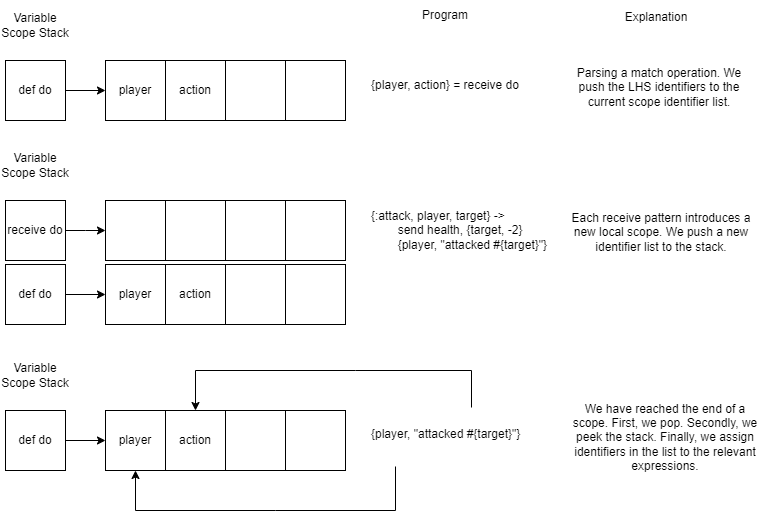
\includegraphics[width=0.9\textwidth]{images/var_stack.drawio.png}
    \caption{Example variable stack and identifier lists. The stack relates to the scope level, we push and pop as we traverse the receive guard. Only values waiting for assignments are added to the identifier list.}
    \label{fig:scope_hierarchy2}
\end{figure}
\subsubsection{Functions, Returning and Recursion}
Like the other constructs, functions introduce a new scope level. Promela does not support functions. We model functions using Promela processes and rendezvous communication channels. To implement functions, we apply various techniques that implement the behaviour of Elixir functions. 
\\ \\
Let's consider a function call. The caller must declare a new communication channel, used to output the return value on. We also declare a new variable to read the return value of the function call, typed using the type specification of the callee. We can now spawn a new process and pass the function arguments, alongside some additional information. 
\\ \\
We first pass the return channel, which is also used for determining whether the callee has terminated. By creating the return channel with a buffer size of 0, the caller will block until the callee returns. We also pass a process identifier. All processes are identified by this process ID; by passing this to the callee, the callee can take actions as if it were communicating as the parent process. We then pass the remaining arguments as if we were making an Elixir function call. 
\\ \\
The caller will now block until the callee sends a message over the return channel. The callee can proceed as normal, and by using the discussed traversal techniques, all exit points will send the final expression over the return channel. This approach easily extends to \textbf{recursion}, as the callee can spawn a new instance of itself and block until a signal is received. In figure \ref{fig:function_call}, we show an example of a recursive function call.
\begin{figure}[h]
    \centering
    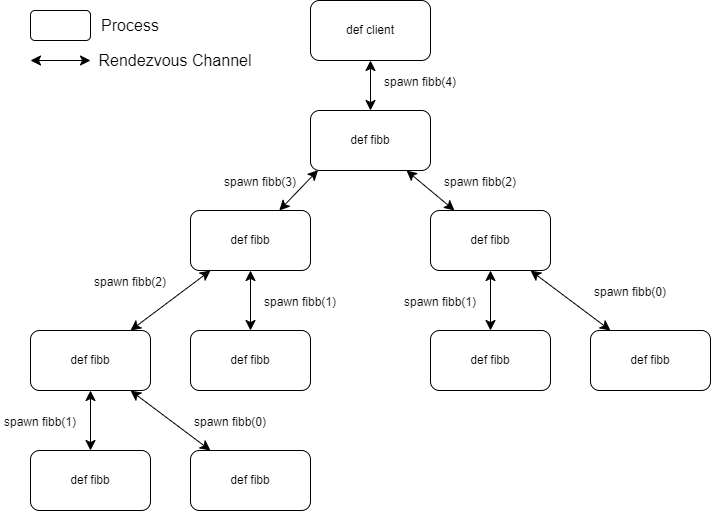
\includegraphics[width=0.8\textwidth]{images/function_call.drawio.png}
    \caption{An example of a recursive function call. In total, 9 processes are spawned to calculate the factorial of 4. Callers block until they rendezvous with callees. If we consider the call stack as a graph, it is traversed in a depth-first manner.}
    \label{fig:function_call}
\end{figure}
\subsection{Concurrent Memory Model} \label{sec:memory_model}
Now we have explored the basics of modelling Elixir programs, we extend the ideas to programs with multiple processes running concurrently. To correctly design a model of a concurrent Elixir system, there are a few core principles we must capture.
\begin{itemize}
    \item Spawning processes.
    \item Sending messages.
    \item Receiving messages.
\end{itemize}
We will first explain how we model the spawning of a new process, before taking a deeper look into more complex concurrency primitives as well as a memory model to extend the existing capabilities of Promela. 
\\ \\
Each Elixir \texttt{function} is already translated to a \texttt{proctype}. We need to tell apart function calls from process spawns. During a spawn, we pass a process identifier to the new child process. In this case, the process identifier is a reserved identifier, which prompts the child to ask the scheduler for a new id. This ensures all parents are uniquely identifiable, which is crucial for communication. The process identifier can be captured in the caller's symbol table and used to communicate with the process.
\subsubsection{Actors, Mailboxes and Message Passing}
Once we have another process's identifier in our symbol table, we can begin communication between processes. To model Elixir actors, we must model the three core components of an actor system: sending, receiving and spawning. We now look at sending and receiving.
\\ \\
\subsubsection{Constructing Messages}
A message is internally comprised of two components: the \textbf{message type} and the \textbf{message body}. When a message type is used in the context of a send or receive it is added to a global set of message types. Tracking this set globally is important to model the entirety of the system. 
\\ \\
The message body consists of multiple message arguments. We can store any primitive type within a message argument by inferring the type from the send or receive expression. If a type cannot be inferred in the context, we reserve a byte array to store the message argument, but to avoid this causing memory issues, we limit the size of the byte array to a small fixed size.
\\ \\
\begin{lstlisting}[language=Promela, caption={Example of a message body, from the Verlixir Promela library.}]
    typedef __message_component {
        byte data1[2];
        int data2;
        byte data3[2];
        bool data4;
        bit data5;
    };
    typedef __message_body {
        __message_component m1;
        __message_component m2;
        __message_component m3;
        ...
    };
\end{lstlisting}
\subsubsection{Sending Messages}
Now that we can construct a message, we can begin to model how messages can be sent and received. Using the global message type set, we construct a mailbox for each message type. The mailboxes are indexed by using a process identifier. We use a \textbf{sorted insert} (!!), so that messages are grouped by their intended target. When a process sends a message, we triage which mailbox the message should be sent to, using the message type and use the process identifier from the symbol table. We also attach the message body to the mailbox. In figure \ref{fig:promela_mailbox}, we show an example of how a mailbox is used.
\\ \\
\begin{figure}[h]
    \centering
    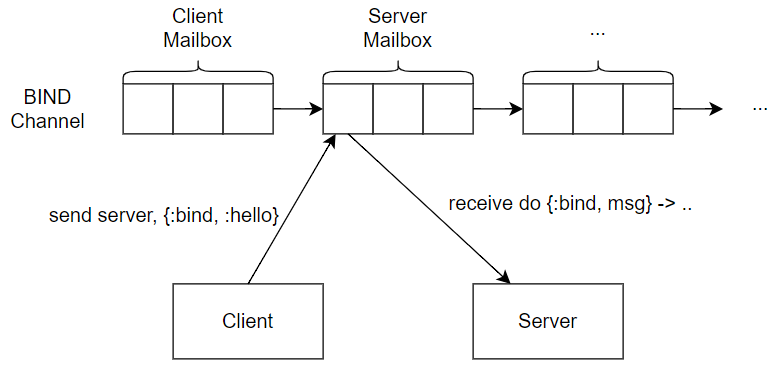
\includegraphics[width=0.8\textwidth]{images/promela_messages.png}
    \caption{An example of modelling the Elixir mailbox.}
    \label{fig:promela_mailbox}
\end{figure}
\\ \\
\subsubsection{Receiving Messages}
Receiving a message is a little more complex. We must now consider pattern matching. To begin pattern matching, we can again use the message type to determine which mailbox to check. If more than just the message type is required in the pattern matching of a guard, we must pre-empt elements of the message body to determine which elements are important for pattern matching and which elements are identifiers that need assignments. 
\\ \\
In order to generate a model for the patterns, we introduce a blocking statement consisting of multiple conditions. When one of the conditions is satisfied (i.e. a message has been pattern-matched), we stop blocking, execute the block relevant for the matched guard and then break out of the control structure. 
\\ \\
Before we can execute the block, we must assign all the remaining identifiers from the receive pattern, to the relevant values in the received message body. To do this, we first introduce a new dummy variable which is assigned the value of the message body. We can then access the dummy variable to assign the remaining identifiers from the guard. During the assignment, we have no indication of the type of the identifier. Hence, we can temporarily assign a message argument to the identifier, and extract the correct attribute from the message argument when we have more information about the type.
\\ \\
Unlike Elixir actors, Verlixir bounds multiple communication primitives. This is to ensure state explosion in the model checker is less likely to occur. As mentioned, we are strict in the bounding of byte arrays that can be passed as message arguments. We also only supply a small number of mailboxes per message type, furthermore, we bound the number of messages that can buffer in a per-process mailbox.
\\ \\
Listing \ref{lst:receive_pattern} shows an example of a receive. We are receiving a $vote$ message. We always match on \texttt{\_\_pid}, to ensure the message is intended for the current process. We read the body into \texttt{\_\_rec\_v\_0} and then extract the individual components. We 
\begin{lstlisting}[language=Promela, caption={Example of a receive pattern. Translation of \texttt{\{:vote, x\}.}}, label={lst:receive_pattern}, xleftmargin=.4\linewidth]
    __message_body __rec_v_0;
    do
    :: __VOTE ?? eval(__pid), __rec_v_0 ->
        __message_component x = __rec_v_0.m1.data2;
        ... body ...
        break;
    od
\end{lstlisting}
\subsubsection{Dynamic Memory Allocation}
Promela does not support dynamic memory allocation. Elixir uses dynamic memory for its structures like lists, maps and sets. The Verlixir Promela library introduces two structures to handle all list operations across the system. Promela supports statically sized arrays. These arrays cannot be passed to other processes. Hence, an array's lifetime is limited to its scope. To get around this limitation, the two structures we introduce are called \texttt{memory} and \texttt{linked\_list}.
\\ \\
First, we describe the design of \texttt{linked\_list}. It is in fact not a traditional linked list, but it behaves similarly, as we can perform many operations on this structure that we could not perform on a statically sized array. For example, we support prepending and appending, which causes dynamic resizes. In actuality, none of these operations resize the list. A list has an upper bound in its size, which is statically set for all model generation. Let's name this limit L.
\begin{lstlisting}[language=C, xleftmargin=.1\linewidth, caption={The structure of a list}.]
typedef __linked_list {
    __node vals[L];
}
\end{lstlisting}
For example for a limit, $10$, means the maximum number of elements that can be appended to the list is 10. The list starts as empty and is handled by the \texttt{node} nested structure.
\begin{lstlisting}[language=C, xleftmargin=.1\linewidth, caption={Example of a list node typed `int'.}]
typedef __node {
    int val;
    bool allocated;
}
\end{lstlisting}
A \texttt{node} stores a single value in a list, as well as a flag to indicate if the value has been allocated. Now, given a sequence of nodes, the order of the nodes represents the order of the Elixir list for all allocated nodes. For example, for a list, ls, $ls[0]$ and $ls[9]$ can be contiguous list elements, if they are both allocated and there are no allocations in between.
\\ \\
Given this representation, we now see why all operations are in linear time. For example, for insertion (prepend or append), we must assign a pointer to a node and iterate through all nodes to find an unallocated node to insert into. We also support many other list operations in the Elixir standard library, all of which use similar logic.
\\ \\
We now extend this implementation to introduce dynamic memory. The implementation is similar to how lists are implemented. We introduce a new field to the \texttt{linked\_list} structure, called \texttt{allocated}. This represents the allocation of a list in memory. We can then similarly introduce memory.
\begin{lstlisting}[language=C, xleftmargin=.1\linewidth, caption={Memory intermediate representation. Limit of M lists.}]
typedef __memory {
    __linked_list lists[M];
}
\end{lstlisting}
We introduce a single, globally defined instance of this structure, named \texttt{\_\_memory}. All processes share this memory for their list allocations. All list operations are treated as a single, indivisible step using \textbf{atomic}. If an Elixir process declares a new list, the IR will allocate a list from memory. The model will iterate through all the lists in memory, to find an unallocated list and return this, as a pointer, to the process. This $pointer$ is generated as an \texttt{int}, which indexes into memory. 
\\ \\
Finally, with all these definitions in place we can support the passing of Elixir lists as function arguments. When we detect a function call, or \texttt{send} expression, passing a list, we first allocate a pointer to a new location in memory. We then copy all the values from the list into the new allocation and then pass the pointer as an argument. With this memory in place, we can now support Elixir lists and operations on them.
\\ \\
\subsubsection{Iteration and Higher Order Functions}
Promela supports for loops, but for our Promela library, these are not sufficient. A \textbf{for comprehension} can be represented as a linear scan through all \texttt{linked\_list} elements. We find the allocated elements and apply the comprehension body to these. We can introduce temporary dummy variables to represent Elixir's \texttt{<-} operator. 
\\ \\
If we want to match on a $for$ comprehension, we must also introduce a pointer into a second \texttt{linked\_list} which tracks new allocations into the matched block independently of the scan through an existing list. A $for$ comprehension over an Elixir range construct, \texttt{n..m}, can be represented with a for loop.
\\ \\
A map operation (such as from the \texttt{Enum} Elixir library) is represented similarly to a $for$ comprehension in the IR. Instead of inlining the body, in order to hold a more fair representation of the Elixir program, dummy anonymous processes are stored to represent higher-order functions.
\\ \\
As a closing note on memory, we describe the representation of randomness. Again, Promela does not inherently support randomness which has influenced the IR design. To represent a function, such as \textbf{random}, from the \texttt{Enum} library, we represent this using multiple truth conditions, which can be selected non-deterministically. One of these conditions will return an allocated list element and one will increment the current list pointer. To ensure termination, if we point to the end of the list before returning a value, we simply return the last allocated value we saw. This is not true randomness, and is not fair to all elements in the list, hence, random operations are strongly discouraged in LTLixir, but are theoretically supported.
\\ \\
Note that as Promela does not support functions, when we generate a model, the Verlixir Promela library is inlined into the model.

\section{Specification Language} \label{sec:specification_language}
LTLixir is a specification language that can be used to reason about the time and change of an Elixir system. This section will primarily discuss the design decisions behind the additional constructs we introduce to Elixir. LTLixir is an Elixir library, built with Elixir's metaprogramming capabilities.
\\ \\
We call any construct prefixed with \texttt{@} a system annotation. All system annotations are treated as ghost variables, meaning they do not affect the runtime of the Elixir program.
\\ \\
\subsection{System Initialisation}
\textbf{@init} marks the entry point for the three operational modes. \texttt{@init} is captured in the intermediate representation; every function marked with \texttt{@init} is instrumented as \textbf{active} in the model. Active processes are spawned in the initial system state.
\\ \\
\subsection{Type Specifications}
For each argument parsed when creating a new function in the IR, we insert a new symbol table entry using the type provided in the type specification. The return type is a special case, as the function could be labelled \textbf{non-returning}. We instrument non-returning functions separately from returning ones.
\\ \\
In returning functions, we must ensure every path the process can take returns a value. Similarly, to ensure function calls calls are handled correctly, a non-returning function must return a dummy value at each exit point. The dummy value is used to rendezvous with the caller, signalling the callee has finished execution.
\subsection{Concurrency Parameters}
A concurrency parameter is a parameter which may cause a change in the behaviour of the system. Every parameter passed to \texttt{@model} is marked as a concurrency parameter in the IR. Instead of parsing the Elixir declaration for the parameter, we assign a reserved \texttt{\_\_PARAM} value to the identifier. The model instrumentor will replace these reserved values with various configurations of the parameter. We discuss how these configurations are generated when we discuss the modes of operation, in section \ref{sec:simulation_verification}.
\\ \\

\subsection{Linear Temporal Logic Formulae}
The specification language supports the introduction of temporal properties through system annotations. The Verlixir library parses these as a string. The model generator will parse the string, and translate it into a Promela LTL formula.
\\ \\
We store a separate symbol table for \textbf{temporal variables}. Temporal variables refer to Elixir variables that are used in LTL formulae. When we parse the program and find the declaration of a temporal variable, we instrument it as a global variable in the model. We now consider this a system property, instead of a property bound to a single process. The Elixir program does not, of course, allow any other processes to modify these variables, so the semantics remain unchanged.
\\ \\
We create a single model for each temporal formula, which allows them to be checked in parallel. This is an important optimisation, as model checking can be computationally expensive. Any non-Elixir constructs used in temporal properties, translate directly into Promela LTL.
\\ \\
The extraction of these properties is in fact a little more complex than explained. We have to consider the nesting of identifiers within Elixir constructs. There is also the possibility that some temporal variables are used as concurrency parameters. There are multiple reasons why local identifiers could conflict when moved to a global context, so conflicts also have to be carefully resolved. To preserve the semantics of the LTL formula, any assignment to a temporal variable must be captured in a single, \textbf{atomic} step. Due to the nature of Elixir's match, capturing this in the model is not trivial.

\subsection{Predicates}
Predicates rely on Elixir's metaprogramming capabilities. A predicate has an identifier and a condition. The condition can be evaluated either at runtime or by the model checker. We implement a \texttt{predicate} as an Elixir \textbf{macro}. Macros are compile-time constructs that are invoked with Elixir's AST as input, and produce a superset of the AST as output. The \texttt{predicate} macro matches the identifier to the condition and inserts it back into the AST. The identifier can be used in any Elixir construct where a condition is expected.
\\ \\
A defined predicate can be used in an LTL formula. We globally define the predicate in the model, such that we can use the predicate identifier in the LTL formula. Given the predicate condition, we must recursively search the condition for any nested identifiers. We move these identifiers to the global scope, and replace the nested identifier with the global identifier. All predicates and nested identifiers are now temporal variables. This step introduces the same complexities as the temporal variables previously discussed.
\subsection{Function Contracts}
A function contract is defined with \texttt{defv}. As with predicates, \texttt{defv} is an Elixir macro, which directly modifies the Elixir AST. Semantically, a contract acts similarly to \texttt{def}. The macro inserts an expression into the AST which contains the function body and \textbf{pre- and post-conditions}. Syntactically, these can be defined using the terms \texttt{pre:} and \texttt{post:} in the function declaration, before the body of the function.
\\ \\
\begin{lstlisting}[language=Elixir, xleftmargin=.1\linewidth, caption={An example contract}.]
defv add_positives(x, y), pre: x > 0 && y > 0, post: ret == x + y do
    ...
end
\end{lstlisting}
The \texttt{defv} macro is intended for verification. It also instruments the execution of Elixir programs, such that at runtime, any violation of a condition will be flagged. This is achieved by capturing the pre- and post-conditions. In the absence of a condition, we insert the \texttt{:ok} atom into the AST. Otherwise, a quoted expression is constructed by first unquoting the condition, evaluating its truth and then possibly flagging a violation. When a call is made to the function, we build a final quoted expression to instrument the call. This final expression consists of the following steps:
\begin{itemize}
    \item We capture a function call and delay the evaluation of the function body.
    \item We evaluate the precondition check.
    \item We evaluate the function body, buffering the result.
    \item We evaluate the postcondition check.
    \item We return the buffered result.
\end{itemize}
Relying on evaluating these conditions at runtime does not prove the correctness of a specification. However, by using contracts with Verlixir, we can ensure function calls and returns are consistent with their specification.
\\ \\
Verlixir models pre- and post-conditions as \textbf{assertions}. Assertions are placed at the entry and exit points of a process. Naturally, the model checker reports assertion violations. We map these assertion violations back to the original Elixir program. The algorithm to determine exit points is the same as we used when returning values. A slight complexity arises if the return value is a non-trivial expression, for example, a receive or if statement. In this case, we must ensure the evaluation of the expression occurs before the post-condition check. This can be complex, as expressions can be nested.
\\ \\

\section{Simulation and Verification} \label{sec:simulation_verification}
We have now explored the intermediate representation constructed by Verlixir, alongside some implementation details specific to using Promela as a target language. This section will describe the remainder of the Verlixir design, which touches on simulation, verification, generating multiple models and using Spin as a target model checker. The default execution of the Verlixir executable, will produce a single Promela model, for a given input LTLixir specification. For Verlixir to produce outputs, it should be executed in an operational mode: $\{-s, -v, -p\}$ for simulation, verification or parameter exploration.
\\ \\
If $-s$ is passed, Spin is run in simulation mode. If $-v$ is passed, Verlixir will first determine the existence of LTL properties within the model. For each LTL property, we run an instance of Spin specifying the LTL property we want to evaluate. We do this using Spin's $-search$ parameter, which will generate and run the verifier from the model. In the event we do not detect an LTL property, we use $-search$ to check for the existence of deadlocks or non-progress cycles (livelocks). If $-p$ is passed, multiple models are generated instead of one, and all of these are checked as if $-v$ was passed for each.
\subsection{Simulation}
Simulation mode will use the Spin scheduler to execute a single execution through the generated state space. A simulation can timeout in the case of a deadlock. If a timeout is produced, we inform the user of the timeout but do not provide further information as that is left for verification mode. Elixir calls to the \texttt{IO} library can be reproduced in simulation mode, as we display them to the user if they are executed. Simulation mode can be more beneficial than examining the output of running an Elixir program. The scheduler takes enabled transitions, based on the current state, whereas, the Elixir scheduler, runs in real-time, which could result in a process interleaving never being observed.
\subsection{Verification}
Verification mode will run the Spin verifier. If an error is detected, the output is captured by the Verlixir error profiler, which triages the issue to generate relevant outputs for the user to digest. For example, if a non-acceptance cycle is produced by Spin, Verlixir captures this and reports to the user that either an LTL property was violated (liveness property) or the system is potentially livelocked. Verlixir will report the entire trace that led to this cycle, showing which process was responsible for a transition between states as well as reading from the Elixir module the line of Elixir code that led to that transition. 
\\ \\
\subsubsection{Reporting Violations}
The mapping between Elixir expressions and how they are modelled is not a one-to-one mapping of line-numbers. Instead a single Elixir expression can result in multiple Promela expressions and multiple states in the state-space Spin traverses. Still, all the relevant Elixir expressions are captured and reported in the trace produced. For this error, Verlixir will also report the cycle that led to non-terminating processes. It will report where the cycle begins, then give a trace of executed Elixir lines and which function executed them. The error profiler also captures and reports the processes which have terminated, or a blocking expression (such as a receive with no accepting guards). For a given model $M$, the profiler can determine the following truth conditions for the specification $\phi$. If the specification holds for an initial state, $S_i$, we have $(M, S_i) \models \phi$. If the specification holds for all initial states, the specification is valid: $M \models \phi$. The error profiler may report a violation, in which case for a violating specification $\phi _v$ we have $(M, S_i) \models \phi _v$. For example, deadlocks, non-accept cycles, out-of-memory, assertion violations are possible violating specifications all represented by $\phi _v \in \{\phi _{dl}, \phi _{cycle}, \phi _{memory}, \phi _{assert}\}$. In the event that $M \models \phi _{memory}$, we could re-run the verification process using directives to reduce memory usage. If this is required, Spin will no longer perform an exhaustive search. If the specification is true under these conditions, we can only say the model partially models the specification, $(M, S_i) \models \phi _p$. A non-exhaustive search should only be applied as a last resort, if it is infeasible to perform verification by reducing the system complexity and can be performed using the $-r$ flag. 
\\ \\
\subsubsection{Fairness}
Similarly, in the event $M \models \phi _{cycle}$, it may be useful to introduce weak fairness to the system. Weak fairness can be applied by passing the $-f$ flag when in verification mode. Other flavours of fairness should be introduced using LTL formulas. If the weak fairness flag is active, scheduling decisions will consider how process-level non-determinism is resolved. For example, if a non-progress cycle is detected by a single process infinitely executing, even when other active processes are not being scheduled, by re-running the verifier with weak fairness applied, infinitely enabled transitions will eventually be scheduled to be taken. This may instead report a new error, consisting of a fair non-progress cycle, or even avoid the non-progress cycle entirely.  
\subsection{Parameterization}
The Verlixir IR passes all detected parameters to the Verlixir model runner. The model runner is responsible for generating multiple models depending on the number of parameters provided, $N$ and the range of search values, $M$, which can be parsed as a command line argument using $-p\text{ }M$. The model runner generates a total of $M^N$ Promela models. All of these models are run in $-search$ mode and violations are reported. Verlixir reports an acceptance score, $\alpha$, determining how many of the models were accepted by the verifier: $\alpha \coloneq 1 - \frac{|V|}{M^N}$, where $V$ are violating models. After outputting $\alpha$, we note all the elements of $V$ so the user can generate a trace for the violation using verification mode.

\section{Modelling Paxos}
We will now demonstrate the model generation process for a larger example, the basic Paxos algorithm. A thorough explanation of the problem will be discussed in section \ref{sec:Paxos}. For now, we will just concern ourselves with the syntax of the Elixir program and how it is parsed and translated into Promela.
\\ \\
The entire program is large, so we will just look at a single Elixir $defmodule$. In particular, we will look at the $learner$ module. When the system is distributed, the $learner$ could be an Elixir node, or an Elixir process. For our model, it does not matter. We will now take a look at the Elixir implementation of one of the functions of the learner, $wait\_learned$, focusing primarily on the syntactic elements.
\\ \\
\begin{lstlisting}[language=Elixir, xleftmargin=.05\linewidth, caption={A function from the $learner$ module}.,label = lst:learner]
@spec wait_learned(list(), integer(), integer()) :: :ok
@ltl """
[]((p->!<>q) && (q->!<>p))
<>(r)
[](s)
"""
def wait_learned(acceptors, p_n, learned_n) do
    predicate p, final_value == 31
    predicate q, final_value == 42
    predicate r, final_value != 0
    predicate s, final_value == 0 || final_value == 31 || final_value == 42

    if p_n == learned_n do
        for acceptor <- acceptors do
            send acceptor, {:terminate}
        end
    else
        receive do
            {:learned, final_value} ->
            IO.puts("Learned final_value:")
            IO.puts(final_value)
        end
        wait_learned(acceptors, p_n, learned_n + 1)
    end
end
\end{lstlisting}
Listing \ref{lst:learner} shows an Elixir function, $wait\_learned$. The function specifies some LTL properties, using the multi-line LTL syntax. The LTL properties rely on the predicates defined in the function body. The function also receives some arguments. In the body, we see a conditional branch, where one branch involves a $for$ comprehension, through a list performing some message sending. The other branch receives a value. At the end of the $else$ condition, we recurse. Let's now break down the Promela model.
\\ \\
\begin{lstlisting}[language=Promela, xleftmargin=.1\linewidth, caption={Promela function definition}., label=lst:func_def]
#define p ((final_value == 31))
#define q ((final_value == 42))
#define r ((final_value != 0))
#define s ((((final_value == 0) || (final_value == 31)) || (final_value == 42)))

proctype wait_learned (int acceptors;int p_n;int learned_n;chan ret;int __pid;int __ret_f) {
    chan ret1 = [1] of { int }; 
    atomic{
        if
        :: __pid == - 1 -> __pid = _pid;
        :: else -> skip;
        fi;
    }
\end{lstlisting}
Listing \ref{lst:func_def} shows the first translation result of Promela from the Elixir function. Firstly, we see the predicates are pulled from the body and placed into the global context.
\\ \\
The function is translated to a process type, named $wait\_learned$. The process receives the same arguments as the Elixir function, using the type specification to type the arguments. Additionally, we receive some meta-arguments $\_\_pid$ and $\_\_ret\_f$. The first line of the function body creates a channel, named $ret1$. Channels of this nature will be used in function calls.
\\ \\
Finally, we see an $atomic$ block, which performs a check on the received $\_\_pid$. If the process ID passed is $-1$, we assign a new process ID from the process scheduler. Otherwise, we continue to act as the caller, by retaining the passed process ID.
Next, we look at the first branch of the Elixir $if$ statement. In particular, we will look at the $for$ comprehension.
\begin{lstlisting}[language=Promela, xleftmargin=.1\linewidth, caption={Promela if statement and for comprehension}., label=lst:for]
if
:: (p_n == learned_n) -> 
    atomic {
        __list_ptr_old = __list_ptr;
        __list_ptr = 0;
        __list_ptr_new = 0;
        do
        :: __list_ptr >= LIST_LIMIT || __list_ptr_new >= LIST_LIMIT -> 
            __list_ptr = __list_ptr_old;
            break;
        :: else -> 
            if
            :: LIST_ALLOCATED(acceptors,__list_ptr) -> 
                int acceptor;
                acceptor = LIST_VAL(acceptors,__list_ptr);
                atomic {
                    MessageList msg_0;
                    __TERMINATE!!acceptor,TERMINATE,msg_0; 
                }
                ;
                __list_ptr_new++;
                __list_ptr++;
            :: else -> __list_ptr++;
            fi
        od
    }
\end{lstlisting}
Listing \ref{lst:for} shows the translation for the $if$ statement. Each condition in the $if$ is determined with a (::) operator. In this listing, we just have the first condition, the $else$ will be seen in a later listing. 
\\ \\
Next, we have the translation of the for comprehension. This is wrapped in an atomic block, as it relies on accessing shared memory. It looks daunting, but all that is taking place is a linear scan through the list. We check each element, determine if it has been assigned and if it has, then the comprehension body (lines 14 through 19) is executed with the list element.
\\ \\
In this case, the comprehension body is a $send$. To send, we pack the message elements into structure, and then send this data to the channel matching our $terminate$ atom, and the mailbox matching $acceptor$.
\\ \\
Now let's look at the $else$ condition.
\begin{lstlisting}[language=Promela, xleftmargin=.1\linewidth, caption={Promela receive and recursion}., label={lst:else}]
:: else -> 
    MessageList rec_v_5;
    do
    :: __LEARNED??eval(__pid),LEARNED,rec_v_5 -> 
        final_value = rec_v_5.m1.data2;
        printf("Learned final_value:\n");
        break;
    od;
    int __temp_cp_arr_2;
    __copy_memory_to_next(__temp_cp_arr_2,acceptors);
    int __ret_placeholder_1;
    run wait_learned(acceptors,p_n,learned_n + 1,ret1,__pid,1);
    ret1?__ret_placeholder_1;
fi;
\end{lstlisting}
Listing \ref{lst:else} shows the translation of the $else$ condition. Again, this is guarded by a (::) operator. We do two things here: first we receive a message and then we recurse.
\\ \\
The receive only has one guard. We translate this guard by reading from the $learned$ channel, looking into our mailbox (marked by \texttt{\_\_pid}). The data we read from the channel is read into \texttt{rec\_v\_5}, which we unpack into the relevant variables.
\\ \\
Secondly, we make a recursive function call. As one of the arguments passed is a list, we must ensure we pass the list by value. To do this, we get a new pointer from memory, and copy the values from our local list into the new memory location.
\\ \\
We next create a value to store the returned value from the recursive call. Actually, in this case the function's type definition marked the function as `non-returning'. We recursively call the function by spawning a new instance of the process type. We pass the parameters, as well as the relevant meta-arguments. In this case, the meta-arguments are:
\begin{itemize}
    \item The channel to send the return value to, $ret1$. This was defined at the beginning of the function body.
    \item We pass our process id, so the spawned function can continue to take actions on our behalf.
    \item We pass $1$. $1$ marks a non-returning function.
\end{itemize}
We then wait to read on $ret1$ to rendezvous with the callee.
\\ \\
Let's finally look at the remaining translated code.
\begin{lstlisting}[language=Promela, xleftmargin=.1\linewidth, caption={Translation of LTL properties}., label={lst:final}]
    atomic  {
        if
        :: __ret_f -> ret!0;
        :: else -> skip;
        fi;
    }
}


ltl ltl_1 { []((p -> ! <> q) && (q -> ! <> p)) };
ltl ltl_2 { <> (r) };
ltl ltl_3 { [](s) };
\end{lstlisting}
Listing \ref{lst:final} shows the remainder of the translated code. To end the function, we have a final $atomic$ block. Within this block, we check the value of the passed $\_\_ret\_f$ value. If this is $1$, the function is non-returning. To handle the resolution of the call stack, we propagate a ghost $0$ through the return channels. If it was a returning function, the return would already have been handled, and hence we can $skip$.
\\ \\
Finally, after the function and back in the global context, we define our LTL properties. We split the multi-line property into multiple properties so they can be checked in parallel. They rely on the predicates defined, which were defined in the global context as they are properties of the system, not a single process.
\\ \\
\section{Summary}
This chapter has discussed some core design concepts behind Verlixir. We first looked at a high-level overview of where the tools fit into a wider toolchain and gave a basic introduction to their architecture. We saw how Elixir was extended using metaprogramming to support inline specifications. We then introduced the core techniques essential to constructing an intermediate representation of a specification, as well as how Promela can be used as a target modelling language for Elixir systems. Finally, we looked at how Verlixir interacts with the model checker Spin to simulate and verify programs while capturing traces of Elixir programs. We will now evaluate the effectiveness of this tooling.
